\subsection{Initial Design}
During initial design meetings it was discussed that each host should have a graph representing the amount of resources (so, most likely CPU usage) each container is using on that host on the home page.

However, it became clear from early drafts of this design, which can be seen in figure \ref{fig:initialDesign}, that this would not display enough hosts without the need for the user to scroll which violates the ``at-a-glance'' requirement of the tool.

If the graphs were responsive, or calculating the values and updating the graphs in real time, it is expected that these graphs would require an unreasonable amount of load on the part of the client (the web browser accessing the website).
This is especially true if the number of hosts were to be as high as initially intended by the PiCloud project.

Additionally, there was no way of knowing, from a glance, which host belonged to which physical tower, which would be useful for diagnosis purposes, for example if a host was disconnected from its power supply. 

It is for these reasons that this design was abandoned.

\begin{figure}[t]
	\centering
	\setlength\fboxsep{0pt}
	\setlength\fboxrule{0.5pt}
	\fbox{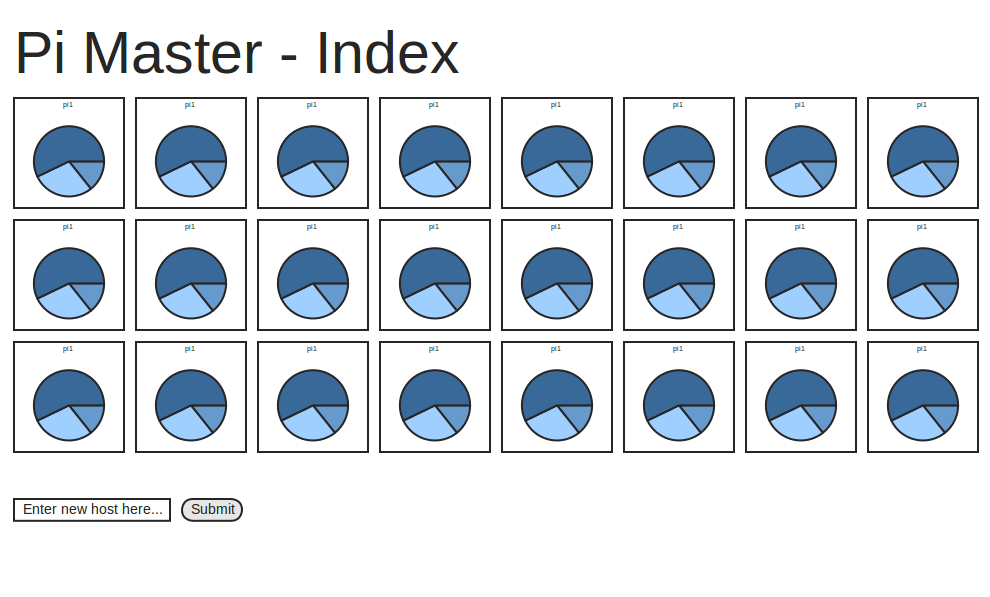
\includegraphics[width=0.8\textwidth]{rmtInitialDesign}}
	\caption{Initial design of \emph{rmt} home page}
	\label{fig:initialDesign}
\end{figure}

\subsection{Refined Design}

Following the lessons learned from the initial design, the home page would now simply list the hosts in such a way as to correspond to the tower they belonged to, and in text rather than graphs.
This would put far less load on the client (web browser accessing the page) and would be able to show more hosts without the need to scroll as much.
The design draft that followed can be seen in figure \ref{fig:refinedDesign}.

Both designs used the same amount of space (1000x600 pixels) yet immediately the user can see 60 hosts in the new design, compared to 24 in the previous design, and there is an immediate distinction between which host belongs to which tower.

\begin{figure}[t]
	\centering
	\setlength\fboxsep{0pt}
	\setlength\fboxrule{0.5pt}
	\fbox{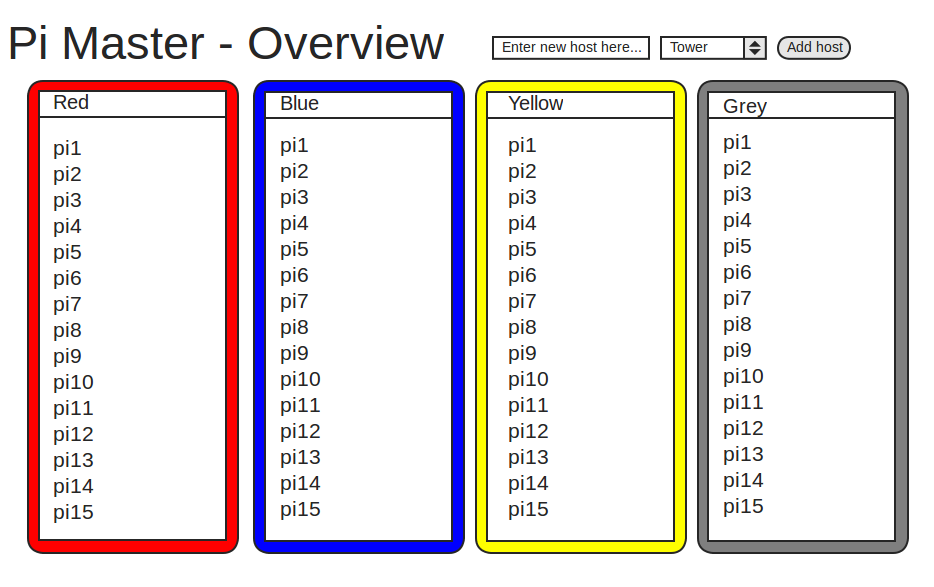
\includegraphics[width=0.8\textwidth]{rmtDesign}}
	\caption{Refined design of \emph{rmt} home page}
	\label{fig:refinedDesign}
\end{figure}